
\sld{Lynxes and Hares}
%
\begin{center}
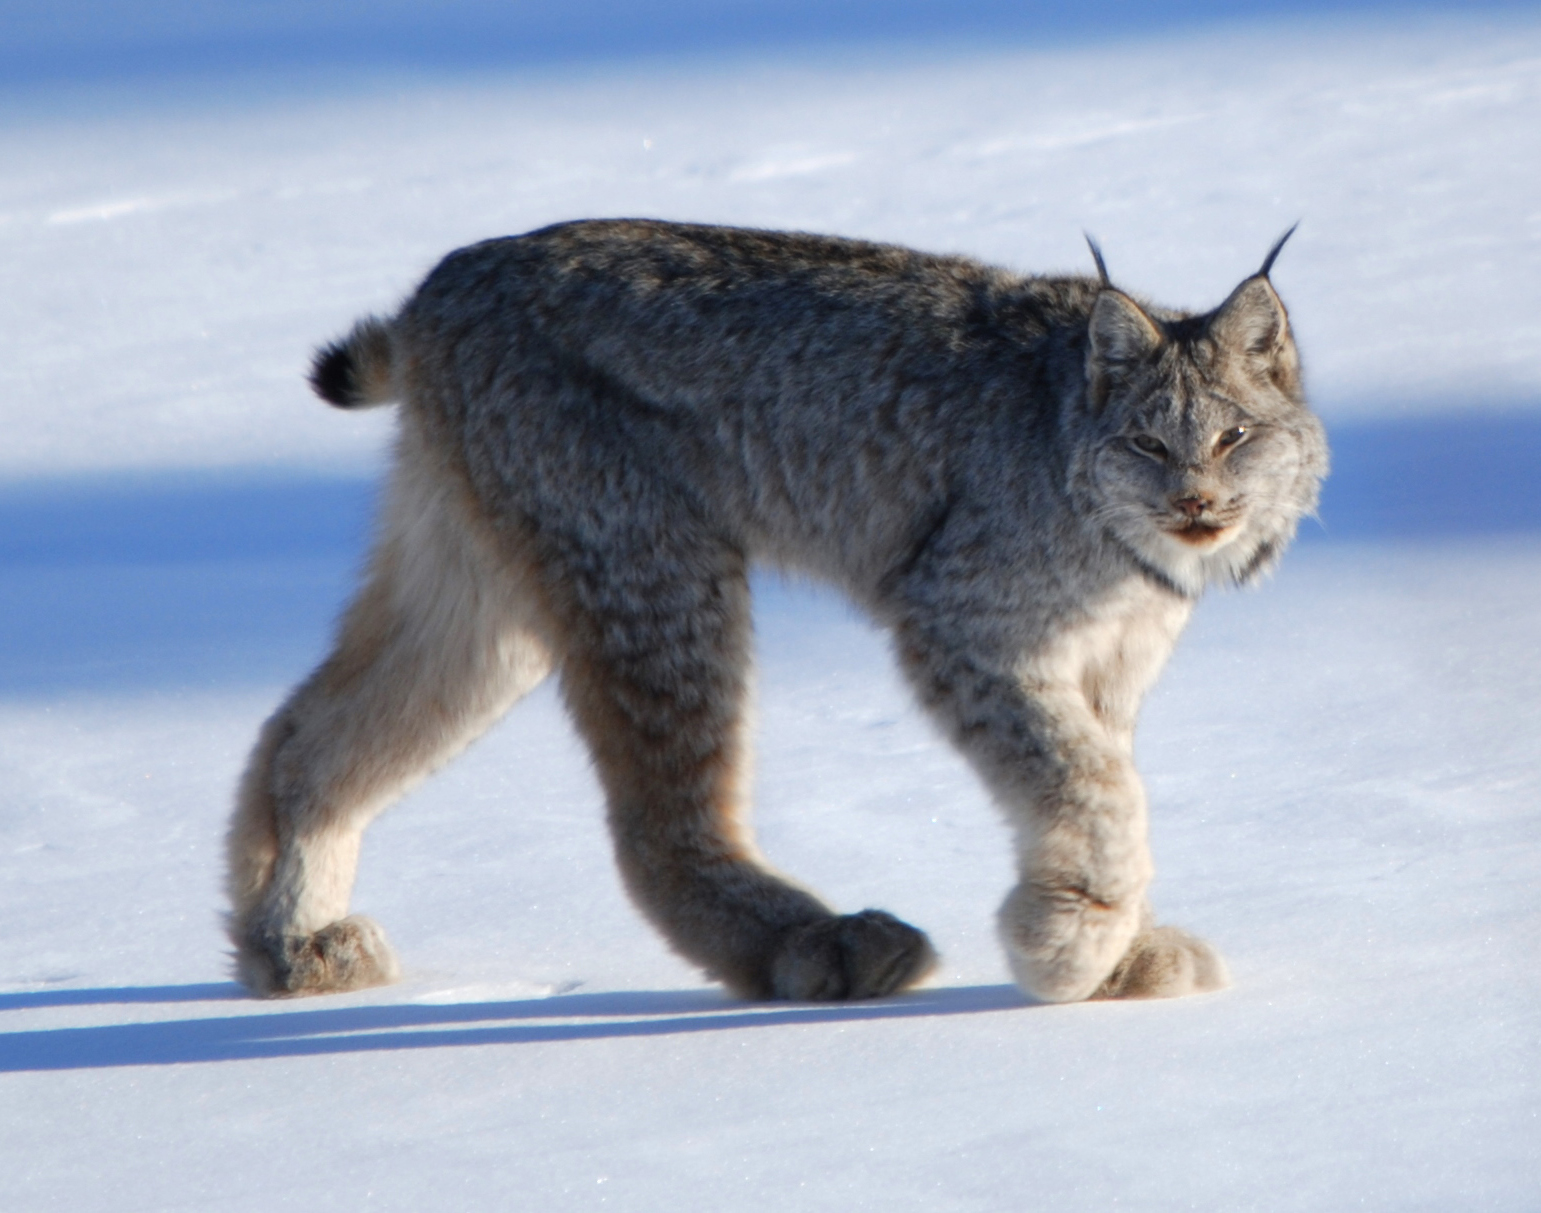
\includegraphics[height=1in]{img/lynx.jpg}
\hspace*{0.25in}
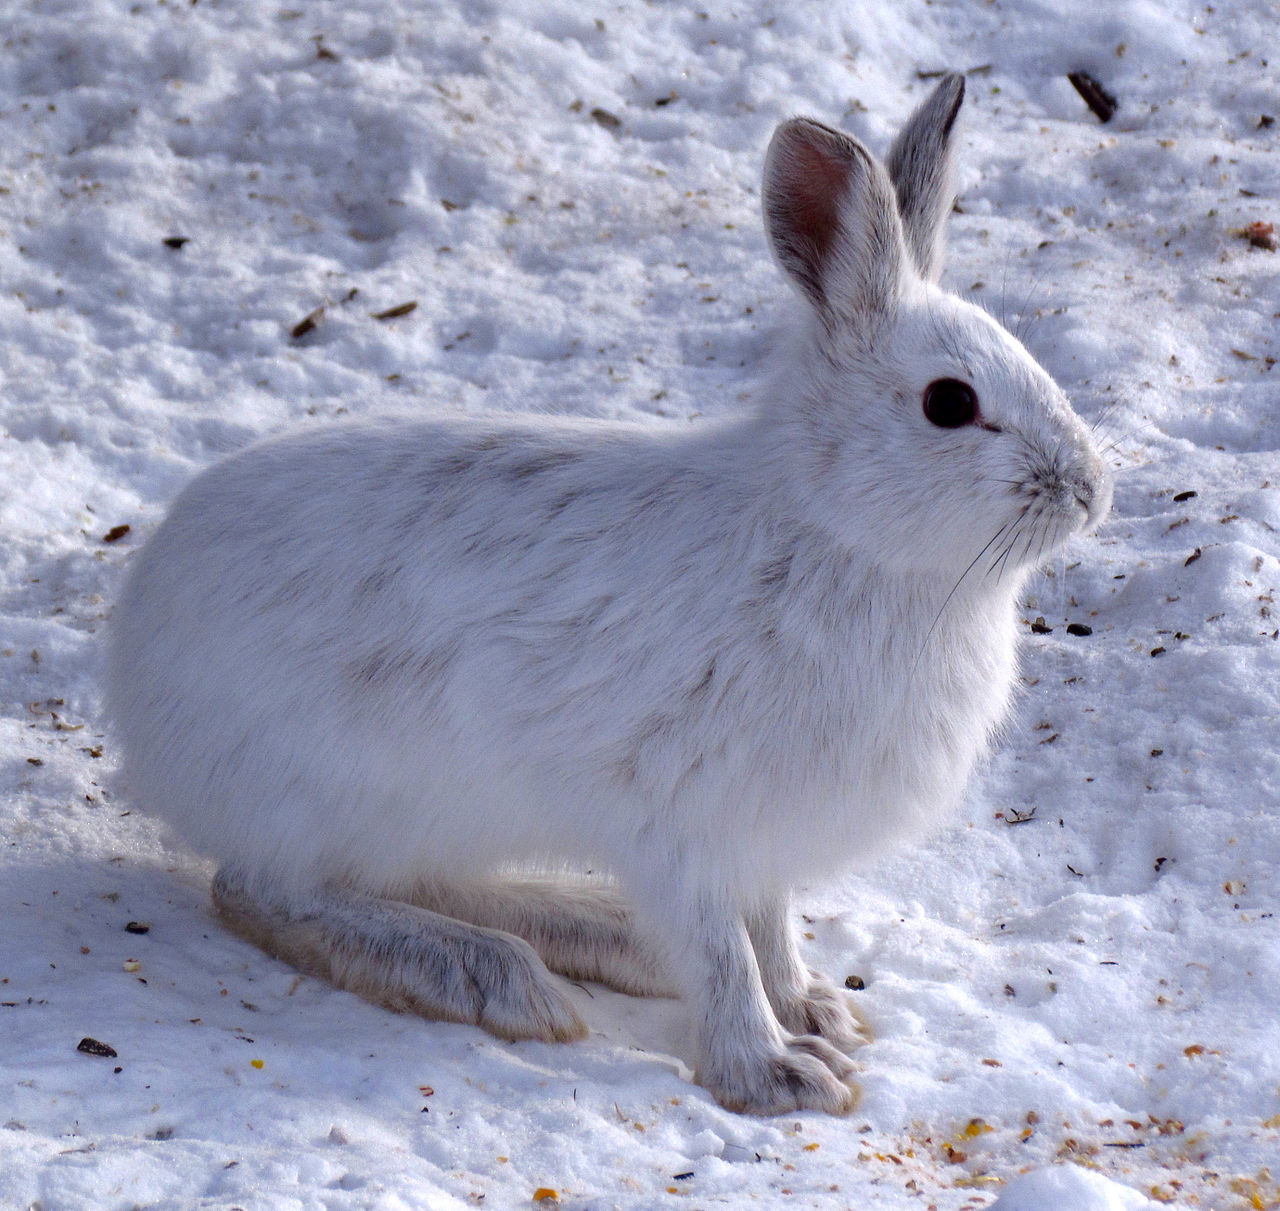
\includegraphics[height=1in]{img/hare.jpg}
\end{center}
\begin{itemize}
\item \myemph{Snowshoe hare} (prey): herbivorous cousin of rabbits
\item \myemph{Canadian lynx} (predator): feline eating primarily hares
\end{itemize}
\vfill
{\tiny
\mbox{ } \hfill
Lynx image copyright 2009, Keith Williams, CC-BY 2.0.
\\[-2pt]
\mbox{ } \hfill
Hare image copyright 2013 D. Gordon E. Robonson, CC-BY SA 2.0}


\sld{Hudson Bay Co. Pelts, 1900--20}
%
\vspace*{6pt}
\begin{center}
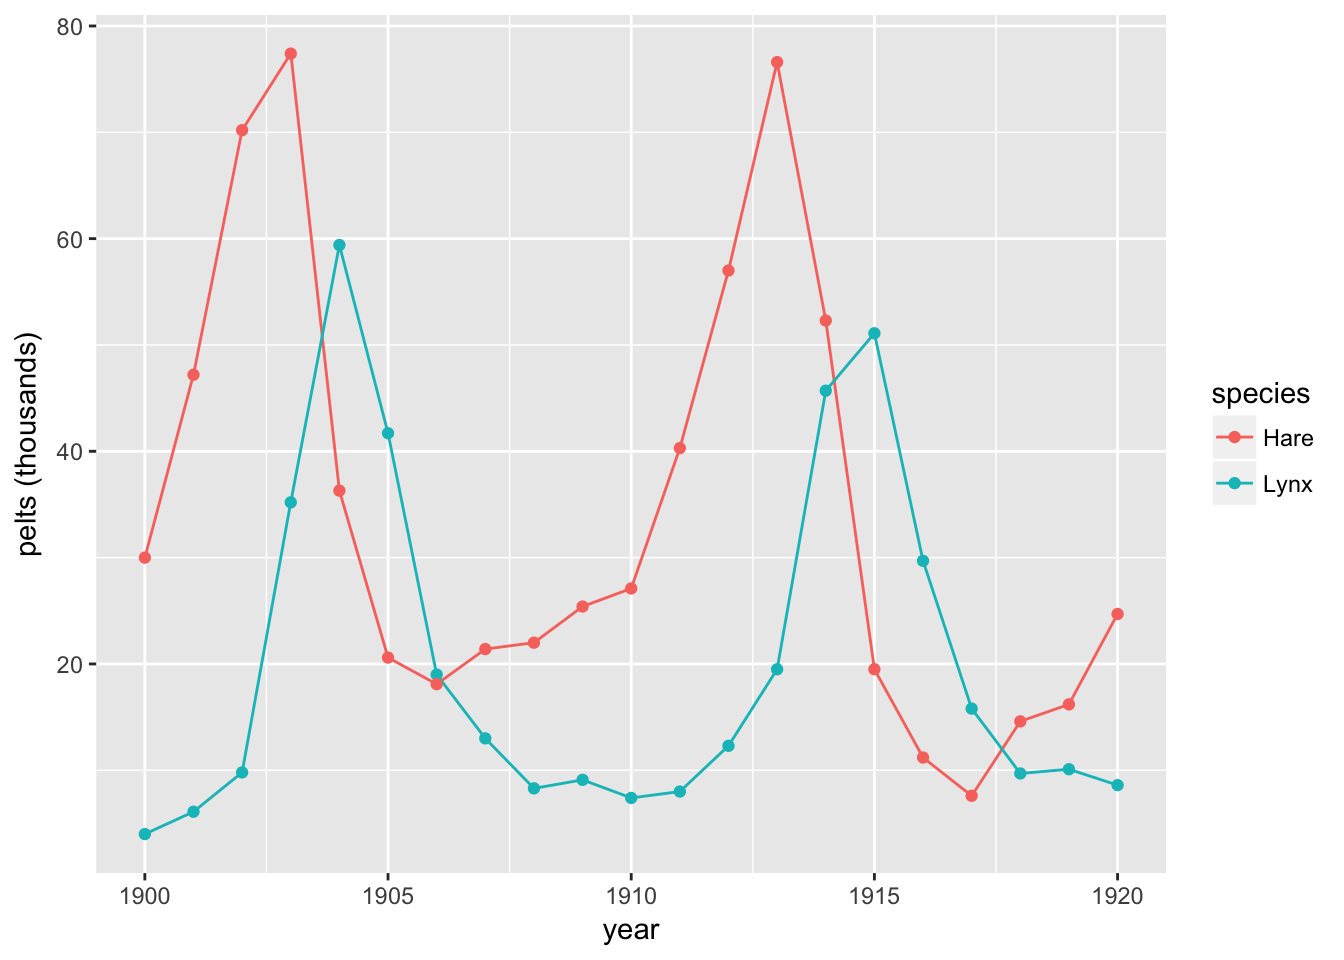
\includegraphics[width=0.6\textwidth]{img/hare-lynx-pelts-1.png}
\end{center}

\sld{Pelts, Phase Space}
%
\vspace*{6pt}
\begin{center}
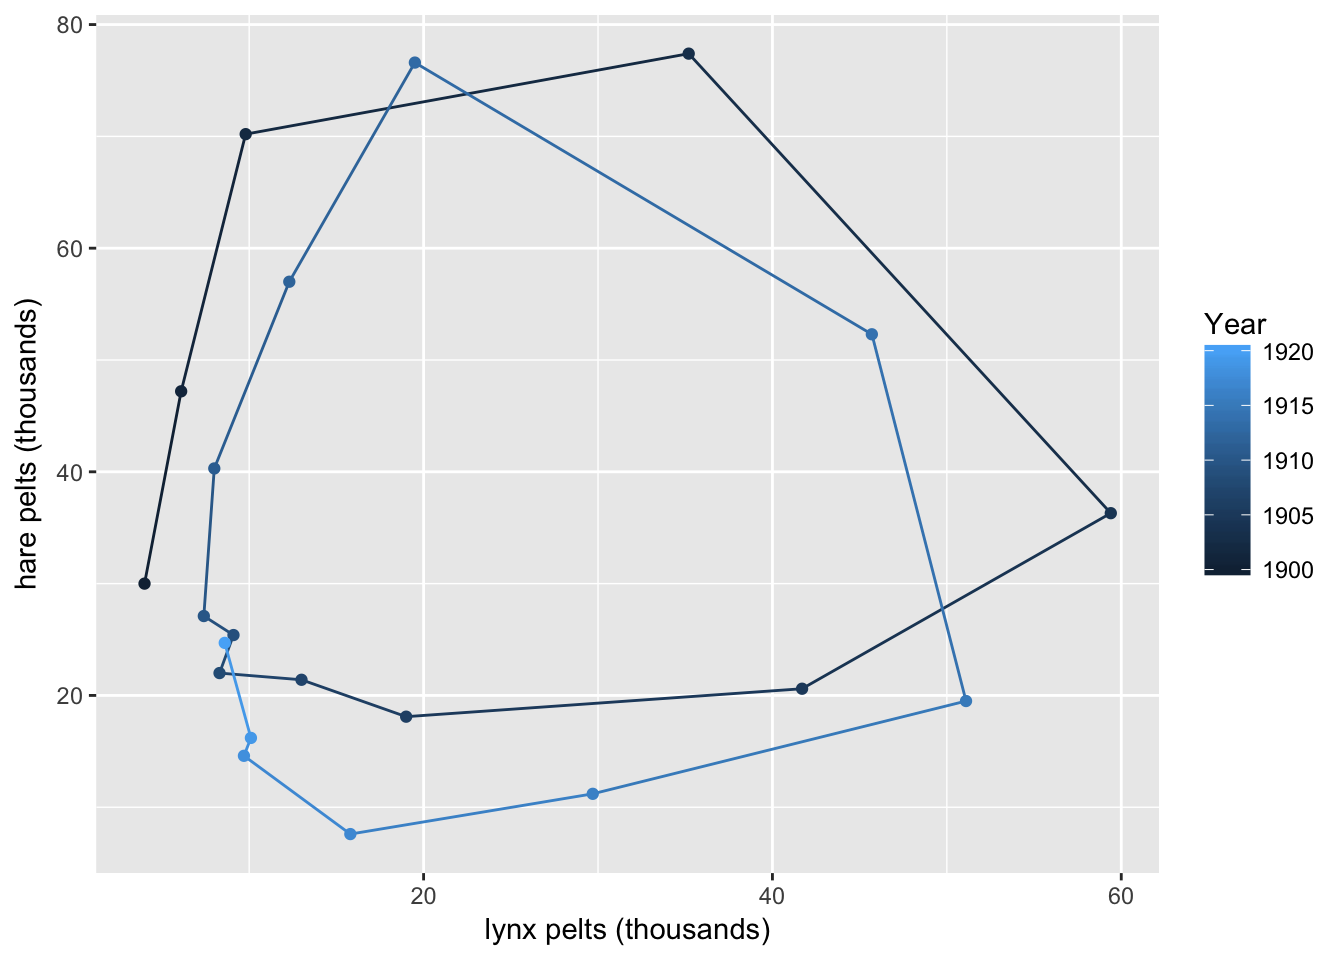
\includegraphics[width=0.6\textwidth]{img/hare-lynx-pelts-2.png}
\end{center}




\sld{\Large Lotka-Volterra in Stan (dynamics)}
%
\vspace*{-2pt}
{\footnotesize
\begin{stancode}
  real[] dz_dt(data real t,       // time (unused)
               real[] z,          // system state
               real[] theta,      // parameters
               data real[] x_r,   // real data (unused)
               data int[] x_i) {  // integer data (unused)
    real u = z[1];            real v = z[2];

    real alpha = theta[1];    real beta = theta[2];
    real gamma = theta[3];    real delta = theta[4];

    real du_dt = (alpha - beta * v) * u;
    real dv_dt = (-gamma + delta * u) * v;
    return { du_dt, dv_dt };
  }
\end{stancode}
}

\sld{Data-Generating Model}
%
\vspace*{-2pt}
\begin{itemize}
\item \myemph{Known} variables are observed
\begin{subitemize}
\item  $y_{n,k}$: pelts for species $k$ at times $t_n$ for $n \in 0:N$
\end{subitemize}
\item \myemph{Unknown} variables must be inferred (\myemph{inverse problem})
\begin{subitemize}
\item initial state: $z^{\mathrm{init}}_k$: initial population for $k$
\item subsequent states $z_{n,k}$: population $k$ at time $t_n$
\item parameters $\alpha, \beta, \gamma, \delta, \sigma > 0$
\end{subitemize}
\item \myemph{Likelihood} assumes errors are proportional (not additive)
\vspace*{-8pt}
\[
y_{n, k} \sim \mathsf{LogNormal}(\hat{z}_{n,k}, \sigma_k),
\]
\vspace*{-4pt}%
{\small where $\hat{z}_n$ is \myemph{solution} at $t_n$ to L-V diff eqs for initial
$z^{\mathrm{init}}$}
\\[-3pt]
\vfill
{\small equivalently: \ $\log y_{n,k} = \log \hat{z}_{n,k} + \epsilon_{n,k}$, \ \ with
$\epsilon_{n,k} \sim \mathsf{Normal}(0, \sigma_k)$}
\end{itemize}


\sld{L-V in Stan (solution to ODE)}
%
\begin{itemize}
\item Define variables for populations predicted by ode, given
\begin{subitemize}
\item system function (\code{dz\_dt}), initial populations (\code{z0})
\item initial time (\code{0.0}), solution times (\code{ts})
\item parameters (\code{theta}), data arrays (unused: \code{rep\_array(...)})
\item tolerances (\code{1e-6}, \code{1-e4}), max iterations (\code{1e3})
\end{subitemize}
\end{itemize}
{\small
\begin{stancode}
transformed parameters {
  real z[N, 2]
    = integrate_ode_rk45(dz_dt, z0, 0.0, ts, theta,
                         rep_array(0.0, 0), rep_array(0, 0),
                         1e-6, 1e-4, 1e3);
}
\end{stancode}
}

\sld{L-V in Stan (data, parameters)}
\begin{itemize}
\item Variables for known constants, observed data
{\footnotesize
\begin{stancode}
data {
  int<lower = 0> N;         // num measurements
  real ts[N];               // measurement times > 0
  real y0[2];               // initial pelts
  real<lower = 0> y[N, 2];  // subsequent pelts
}
\end{stancode}
}
\item Variables for unknown parameters
{\footnotesize
\begin{stancode}
parameters {
  real<lower = 0> theta[4];  // alpha, beta, gamma, delta
  real<lower = 0> z0[2];     // initial population
  real<lower = 0> sigma[2];  // scale of prediction error
}
\end{stancode}
}
\end{itemize}

\sld{L-V in Stan (priors, likelihood)}
%
\vspace*{-6pt}
\begin{itemize}
\item Sampling statements for priors and likelihood
\begin{stancode}
model {
  // priors
  sigma ~ lognormal(0, 0.5);
  theta[{1, 3}] ~ normal(1, 0.5);  theta[{2, 4}] ~ normal(0.05, 0.05);

  z0[1] ~ lognormal(log(30), 5);  z0[2] ~ lognormal(log(5), 5);

  // likelihood (lognormal)
  for (k in 1:2) {
    y0[k] ~ lognormal(log(z0[k]), sigma[k]);
    y[ , k] ~ lognormal(log(z[, k]), sigma[k]);
  }
}
\end{stancode}
\end{itemize}

\sld{\Large Lotka-Volterra Posterior Predictions}
%
\vspace*{-4pt}
\begin{center}
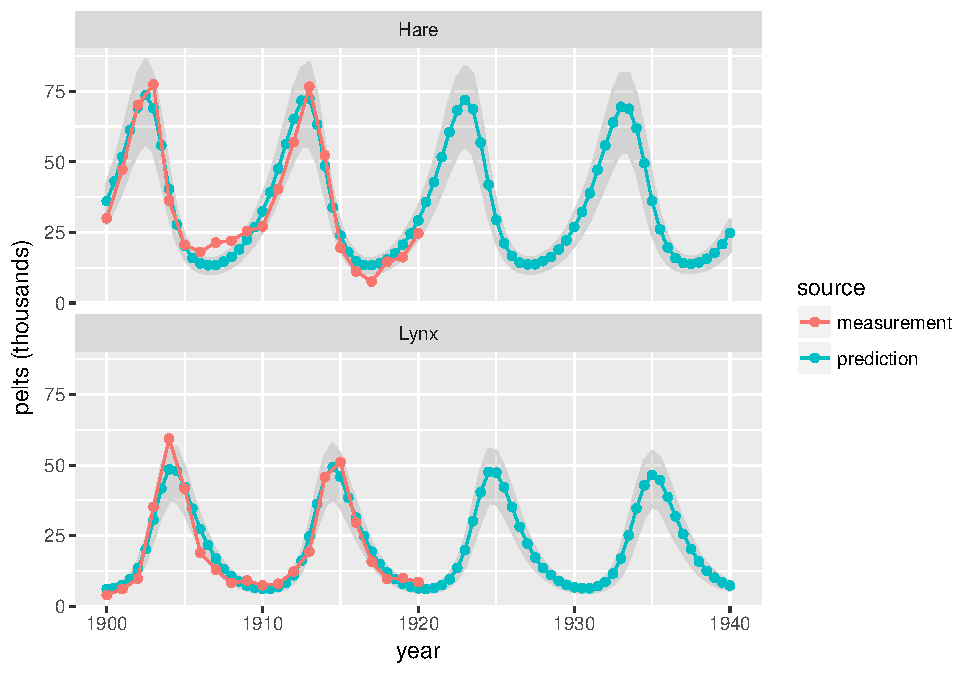
\includegraphics[width=0.525\textwidth]{img/lotka-volterra-predict.pdf}
\end{center}
\vspace*{-6pt}
\begin{subsubitemize}
\item did not include \texttt{generated quantities} block---just more of same
\item training data (1900-1920); \ future predictions (1921+)
\end{subsubitemize}
